\chapter{Conservación de la energía.}
\section{Definiciones.}
\begin{itemize}
	\item Presión de remanso:
	\[P_0=P+\rho\dfrac{v^2}{2}\]
	\item Entalpía de remanso:
	\[h_0=h+\dfrac{v^2}{2}\rightarrow h= e +\dfrac{P}{\rho}\]
	\item Bernoulli:
	\[P_0+U=cte\]
	
	Donde $e$ es la energía interna.
\end{itemize}
\section{Conservación de la energía en forma integral.}
La expresión genérica de la conservación de la energía para un volumen fluido:
\[
\red{\underbrace{\black 
\dfrac{D}{Dt}\iiint_{V_f}\rho \left(e+\dfrac{v^2}{2}\right)\,dV
}_{\text{Variación de energía interna, $e$}}} \black
=
\red{\underbrace{\black
\oiint_{S_f}-P\left(\vec{v}\cdot \vec{n}\right)\,dS
+
\oiint_{S_f}\vec{v}\cdot\overline{\overline{\tau}}\cdot \vec{n}\,dS
+
\iiint_{V_f}\vec{f}_v\cdot \vec{v}\,dV
}_{\text{Trabajo}}} \black
+
\red{\underbrace{\black
\oiint_{S_f}-\vec{q}\cdot \vec{n}\,dS
}_{\text{Calor por conducción}}} \black
+
\text{Otras energías}\]

El calor transferido por conducción para un líquido perfecto newtoniano se puede expresar mediante la siguiente ecuación ($e=C_P\cdot T$ y $K=cte$):
\[\rho C_P\dfrac{\partial T}{\partial t} 
+ 
\rho C_P\left(\vec{v}\cdot\vec{\nabla}T\right)
=
K\vec{\nabla}^2T
+
\red{\underbrace{\black
\left\langle
	 2\overline{\overline{\tau}},
	 \dfrac{1}{2}\left[\vec{\nabla}\vec{v}+\left(\vec{\nabla}\vec{v}\right)^t\right]
\right\rangle
}_{\substack{\text{Función de disipación de Raleigh. }
\\ \text{$ \left\langle , \right\rangle $ denota el operador producto interno.}}}} \black
\]


No obstante, antes de resolver esta ecuación, para obtener el campo de velocidades, $\vec{v}$, han de resolverse las ecuaciones de conservación de la masa y de cantidad de movimiento.
\[\left\{
\begin{matrix}
	\vec{\nabla}\cdot\vec{v}=0 \\
	\rho\dfrac{\partial \vec{v}}{\partial t}+\rho\left(\vec{v}\cdot\vec{\nabla}\right)\vec{v}=-\vec{\nabla}P+\mu\vec{\nabla}^2\vec{v}+ \vec{f}_v
\end{matrix}
\right.\]


Para simplificar los problemas, en la asignatura se trabaja con casos aislados térmicamente, es decir, debe cumplirse que:
\[\oiint_{S_f}-\vec{q}\cdot \vec{n}\,dS+\text{Otras energías}\approx 0\]
Particularizando al volumen de control que queda encerrado por la entrada, la salida, la pared del conducto y las posibles máquinas rotativas que pudiese haber:
\begin{figure}[H]
	\centering
		\begin{circuitikz}
			\tikzstyle{every node}=[font=\LARGE]
			\draw [ color={rgb,255:red,255; green,0; blue,0} , dashed] (1.5,12.5) rectangle  (11.5,8.5);
			\draw [ color={rgb,255:red,255; green,0; blue,0} , dashed] (6,10.5) circle (1.5cm);
			\draw [short] (1.25,12.75) -- (11.75,12.75);
			\draw [short] (1.25,8.25) -- (11.75,8.25);
			\draw  (6,10.5) circle (1.4cm) node {\normalsize Maquina rotativa} ;
			\node [font=\normalsize, color={rgb,255:red,255; green,0; blue,0}] at (11,12) {$V_c$};
			\node [font=\normalsize] at (1,10.5) {$S_e$};
			\node [font=\normalsize] at (11.75,10.25) {$S_s$};
			\node [font=\normalsize] at (7.75,10.5) {$S_m$};
			\node [font=\normalsize] at (6.75,13) {$S_p$};
		\end{circuitikz}
		\caption{Diagrama genérico de un posible conducto.}
	\label{fig:my_label}
\end{figure}

\[\dfrac{d}{dt}\iiint_{V_c} \rho \left(e+\dfrac{v^2}{2}\right)\,dV
+
\oiint_{S_c} \rho \left(e+\dfrac{v^2}{2}\right)\left(\vec{v}-\vec{v}_c\right)\cdot\vec{n}\,dS
=
\red{\underbrace{\black
\oiint_{S_c} -P\left(\vec{v}\cdot\vec{n}\right)\,dS
}_{\text{Trabajo máquinas rotativas}}} \black
+
\oiint_{S_c}\vec{v} \cdot\overline{\overline{\tau}}\cdot\vec{n}\,dS
+
\iiint_{V_c}\vec{f}_v\cdot \vec{v}\,dV
\]

\section{Bombas/compresores y turbinas.}
\begin{itemize}
	\item Cuando se trabaja con gases el trabajo ideal desarrollado por un compresor es:
	\[\dot{W}_C=G(h_{0_s}-h_{0_e})\]
	
	Donde $G$ es el gasto y por conservación de la masa se puede expresar en magnitud de entrada o de salida.
	\[G=\rho_e A_e v_e=\rho_s A_s v_s\]
	
	\item Cuando se trabaja con líquidos el trabajo ideal desarrollado por una bomba es:
	\[\dot{W}=Q(P_{0_s}-P_{0_e})\]
\end{itemize}

El criterio de signos del trabajo es:
\begin{itemize}
	\item $\dot{W}>0$ para bombas y compresores.
	\item $\dot{W}<0$ para turbinas.
\end{itemize}


Si se trabaja con máquinas reales, cuando se habla del trabajo real, se refiere al trabajo que sería necesario aportar o que se recibiría de la máquina teniendo en cuenta su rendimiento. Por ello:
\begin{itemize}
	\item $\dot{W}_{B_{Real}}=\dfrac{\dot{W}_{B_{ideal}}}{\eta_B}$, se debe aportar más energía para realizar el trabajo útil.
	\item $\dot{W}_{C_{Real}}=\dfrac{\dot{W}_{C_{ideal}}}{\eta_C}$, se debe aportar más energía para realizar el trabajo útil.
	\item $\dot{W}_{T_{Real}}=\dot{W}_{T_{ideal}}\cdot \eta_T$, el trabajo obtenido a través de la turbina es menor debido a las pérdidas.
\end{itemize}
\section{Pérdidas de carga.}
Cuando el fluido pasa por codos, descarga a conducto o ensancha de forma brusca se producen pérdidas en la presión de remanso. Para modelarlo, se emplea un factor $K_P$ de pérdidas. La velocidad máxima se elige la mayor entra la entrada y la salida.0
\[P_{0_e}+\rho U_e=P_{0_s}+\rho U_s+K_P \dfrac{\rho v^2_{max}}{2}\]
\begin{figure}[H]
	\centering
		\begin{circuitikz}
			\tikzstyle{every node}=[font=\normalsize]
			\draw [short] (0.25,10) -- (1.5,10);
			\draw [short] (1.5,10) -- (2.75,10.75);
			\draw [short] (0.25,9) -- (1.5,9);
			\draw [short] (1.5,9) -- (3,10.25);
			\draw [dashed] (3.75,11.75) -- (3.75,8);
			\draw [short] (7.25,10.75) -- (5.5,10);
			\draw [short] (5.5,9.5) -- (7.25,9);
			\draw [short] (5.5,10) -- (4.5,10);
			\draw [short] (4.5,9.5) -- (5.5,9.5);
			\draw [dashed] (8,8) -- (8,11.75);
			\draw [short] (8.75,10.75) -- (8.75,9);
			\draw [short] (8.75,9) -- (10,9);
			\draw [short] (10,9.25) -- (10,8.75);
			\draw [short] (10.5,8.75) -- (10.5,9.25);
			\draw [short] (10.5,9) -- (11.5,9);
			\draw [short] (11.5,9) -- (11.5,10.75);
			\node at (1.25,9.5) [circ, color={rgb,255:red,255; green,0; blue,0}] {};
			\node at (2,10) [circ, color={rgb,255:red,255; green,0; blue,0}] {};
			\node at (5.25,9.75) [circ, color={rgb,255:red,255; green,0; blue,0}] {};
			\node at (6,9.75) [circ, color={rgb,255:red,255; green,0; blue,0}] {};
			\node at (10.25,9.5) [circ, color={rgb,255:red,255; green,0; blue,0}] {};
			\node at (10.25,8.5) [circ, color={rgb,255:red,255; green,0; blue,0}] {};
			\node [font=\normalsize, color={rgb,255:red,255; green,0; blue,0}] at (1,9.5) {e};
			\node [font=\normalsize, color={rgb,255:red,255; green,0; blue,0}] at (4.75,9.75) {e};
			\node [font=\normalsize, color={rgb,255:red,255; green,0; blue,0}] at (10.25,9.75) {e};
			\node [font=\normalsize, color={rgb,255:red,255; green,0; blue,0}] at (2.25,10) {s};
			\node [font=\normalsize, color={rgb,255:red,255; green,0; blue,0}] at (6.25,9.75) {s};
			\node [font=\normalsize, color={rgb,255:red,255; green,0; blue,0}] at (10.25,8.25) {s};
		\end{circuitikz}
	\caption{Ejemplos de regiones con pérdidas de carga.}
	\label{fig:my_label}
\end{figure}
\section{Factor de fricción (f).}
Cuando se trata de tubos en lugar de haber un factor de pérdidas en carga, para caracterizar las pérdidas suele existir una función f. La función f indica la rugosidad relativa.
\begin{itemize}
	\item Si se trabaja en flujo laminar en tubo circular $f=\dfrac{64}{Re_D}$.
	\item Si se trabaja con flujo turbulento completamente desarrollado, para obtener su valor se consulta el ábaco de Moody \ref{fig:moody} donde se obtiene el valor a partir del número de Reynolds.
\end{itemize}

\begin{figure}[H]
	\centering

		\begin{circuitikz}
			\tikzstyle{every node}=[font=\normalsize]
			\draw [short] (0.25,13) -- (10.5,13);
			\draw [short] (0.25,11.5) -- (10.5,11.5);
			\draw [ color={rgb,255:red,255; green,0; blue,0} ] (3.25,11.5) circle (0.5cm);
			\draw [ color={rgb,255:red,255; green,0; blue,0}, ->, >=Stealth, dashed] (6.25,9.5) -- (3.75,11.25);
			\draw [ color={rgb,255:red,255; green,0; blue,0} ] (7.5,8.25) circle (1.75cm);
			\draw [short] (5.75,8.25) -- (6,8.5);
			\draw [short] (6,8.5) -- (6.25,7.75);
			\draw [short] (6.25,7.75) -- (6.25,8.75);
			\draw [short] (6.25,8.75) -- (6.5,7.75);
			\draw [short] (6.5,7.75) -- (6.5,9.25);
			\draw [short] (6.5,9.25) -- (6.75,8.5);
			\draw [short] (6.75,8.5) -- (7,8.25);
			\draw [short] (7,8.25) -- (7,8.5);
			\draw [short] (7,8.5) -- (7.25,8.25);
			\draw [short] (7.25,8.25) -- (7.5,8.5);
			\draw [short] (7.5,8.5) -- (7.75,8.25);
			\draw [short] (7.75,8.25) -- (8,8.5);
			\draw [short] (8,8.5) -- (8,8.25);
			\draw [short] (8,8.25) -- (8.5,8.75);
			\draw [short] (8.5,8.75) -- (8.75,7.75);
			\draw [short] (8.75,7.75) -- (9,8.25);
			\draw [short] (9,8.25) -- (9.25,8.5);
		\end{circuitikz}
	\caption{Representación de la rugosidad en un tubo.}
	\label{fig:my_label}
\end{figure}

Cuando se dedujo la expresión de Bernoulli, se igualó a cero al no existir pérdidas. No obstante, la expresión si se introducen las pérdidas es:
\[\dfrac{\partial}{\partial z}\left(P+\rho\dfrac{v^2}{2}+\rho U\right)=-\rho f\dfrac{v|v|}{8 r.h.}\]

Donde $r.h.$ es el radio hidraúlico ($r_h$): 
\[r.h.=r_h=\dfrac{\text{Área de paso}}{\text{Perímetro mojado}}\xrightarrow{\text{Sección circular}} r.h.=r_h=\dfrac{\pi D^2/4}{\pi D}=\dfrac{D}{4} \]

Por tanto:
\[\dfrac{\partial}{\partial z}\left(P+\rho\dfrac{v^2}{2}+\rho U\right)=-\rho f\dfrac{v|v|}{2D}\]


Integrando en $z=0\rightarrow L$ e ignorando la dirección del flujo (el criterio de signos se elige cuando se hace el problema):
\[\left[P_e+\rho\dfrac{v_e^2}{2}+\rho U_e\right]-\left[P_s+\rho\dfrac{v_s^2}{2}+\rho U_s\right]=\rho f\dfrac{v^2L}{2D}\]


Por tanto:
\[K_{P_{long}}=f\dfrac{L}{D}\]

\subsection{Ecuación de Euler-Bernoulli}
Si se tiene en cuenta el término local:
\[\rho\dfrac{\partial v}{\partial t}+\dfrac{\partial}{\partial z}\left(P+\rho\dfrac{v^2}{2}+\rho U\right)=-\rho f\dfrac{v|v|}{8 r.h.}\]
\section{Ábaco de Moody.}
\begin{figure}[H]
	\centering
	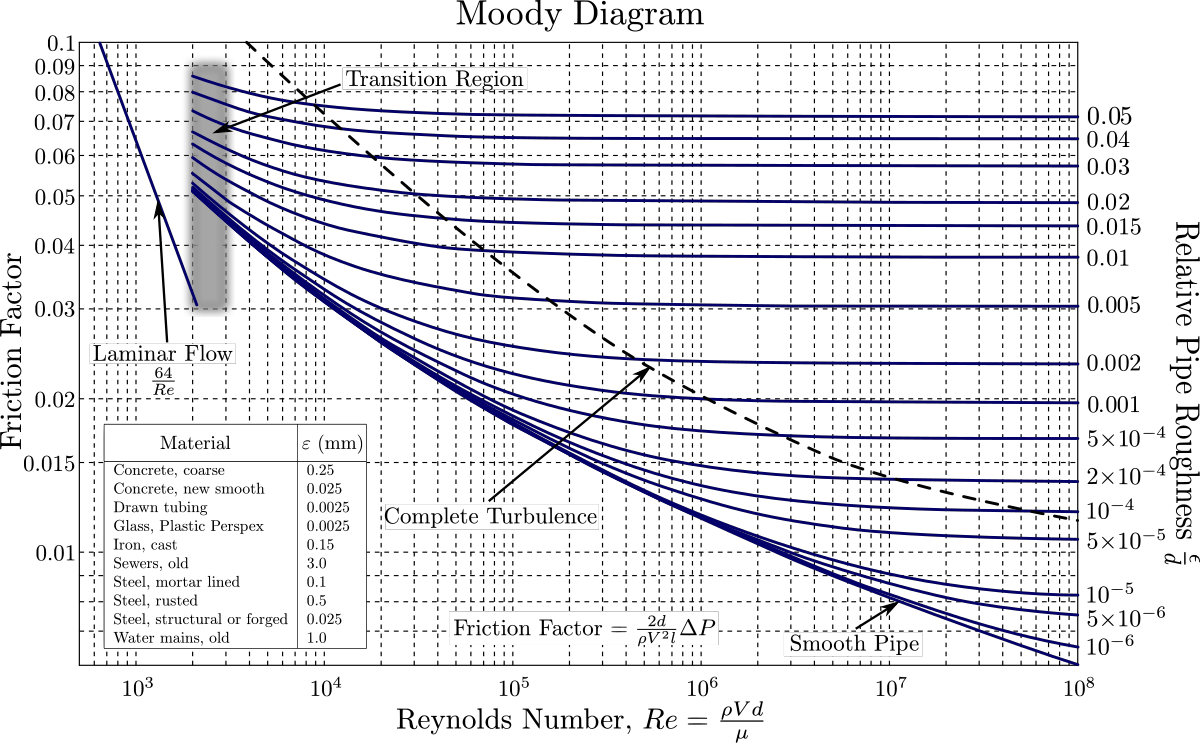
\includegraphics[width=1\linewidth]{ImagenesTema6/Moody}
	\caption{Diagrama de Moody.}
	\label{fig:moody}
\end{figure}
